% Options for packages loaded elsewhere
\PassOptionsToPackage{unicode}{hyperref}
\PassOptionsToPackage{hyphens}{url}
%
\documentclass[
  english,
  man]{apa6}
\usepackage{lmodern}
\usepackage{amssymb,amsmath}
\usepackage{ifxetex,ifluatex}
\ifnum 0\ifxetex 1\fi\ifluatex 1\fi=0 % if pdftex
  \usepackage[T1]{fontenc}
  \usepackage[utf8]{inputenc}
  \usepackage{textcomp} % provide euro and other symbols
\else % if luatex or xetex
  \usepackage{unicode-math}
  \defaultfontfeatures{Scale=MatchLowercase}
  \defaultfontfeatures[\rmfamily]{Ligatures=TeX,Scale=1}
\fi
% Use upquote if available, for straight quotes in verbatim environments
\IfFileExists{upquote.sty}{\usepackage{upquote}}{}
\IfFileExists{microtype.sty}{% use microtype if available
  \usepackage[]{microtype}
  \UseMicrotypeSet[protrusion]{basicmath} % disable protrusion for tt fonts
}{}
\makeatletter
\@ifundefined{KOMAClassName}{% if non-KOMA class
  \IfFileExists{parskip.sty}{%
    \usepackage{parskip}
  }{% else
    \setlength{\parindent}{0pt}
    \setlength{\parskip}{6pt plus 2pt minus 1pt}}
}{% if KOMA class
  \KOMAoptions{parskip=half}}
\makeatother
\usepackage{xcolor}
\IfFileExists{xurl.sty}{\usepackage{xurl}}{} % add URL line breaks if available
\IfFileExists{bookmark.sty}{\usepackage{bookmark}}{\usepackage{hyperref}}
\hypersetup{
  pdftitle={Reproduction of the Analysis of Experiment 1 of Mehr, Song, \& Spelke (2016): For 5-Month-Old Infants, Melodies Are Social},
  pdfauthor={Liat Kofler1},
  pdflang={en-EN},
  pdfkeywords={Social infomation, Infants, Melodies},
  hidelinks,
  pdfcreator={LaTeX via pandoc}}
\urlstyle{same} % disable monospaced font for URLs
\usepackage{graphicx,grffile}
\makeatletter
\def\maxwidth{\ifdim\Gin@nat@width>\linewidth\linewidth\else\Gin@nat@width\fi}
\def\maxheight{\ifdim\Gin@nat@height>\textheight\textheight\else\Gin@nat@height\fi}
\makeatother
% Scale images if necessary, so that they will not overflow the page
% margins by default, and it is still possible to overwrite the defaults
% using explicit options in \includegraphics[width, height, ...]{}
\setkeys{Gin}{width=\maxwidth,height=\maxheight,keepaspectratio}
% Set default figure placement to htbp
\makeatletter
\def\fps@figure{htbp}
\makeatother
\setlength{\emergencystretch}{3em} % prevent overfull lines
\providecommand{\tightlist}{%
  \setlength{\itemsep}{0pt}\setlength{\parskip}{0pt}}
\setcounter{secnumdepth}{-\maxdimen} % remove section numbering
% Make \paragraph and \subparagraph free-standing
\ifx\paragraph\undefined\else
  \let\oldparagraph\paragraph
  \renewcommand{\paragraph}[1]{\oldparagraph{#1}\mbox{}}
\fi
\ifx\subparagraph\undefined\else
  \let\oldsubparagraph\subparagraph
  \renewcommand{\subparagraph}[1]{\oldsubparagraph{#1}\mbox{}}
\fi
% Manuscript styling
\usepackage{upgreek}
\captionsetup{font=singlespacing,justification=justified}

% Table formatting
\usepackage{longtable}
\usepackage{lscape}
% \usepackage[counterclockwise]{rotating}   % Landscape page setup for large tables
\usepackage{multirow}		% Table styling
\usepackage{tabularx}		% Control Column width
\usepackage[flushleft]{threeparttable}	% Allows for three part tables with a specified notes section
\usepackage{threeparttablex}            % Lets threeparttable work with longtable

% Create new environments so endfloat can handle them
% \newenvironment{ltable}
%   {\begin{landscape}\begin{center}\begin{threeparttable}}
%   {\end{threeparttable}\end{center}\end{landscape}}
\newenvironment{lltable}{\begin{landscape}\begin{center}\begin{ThreePartTable}}{\end{ThreePartTable}\end{center}\end{landscape}}

% Enables adjusting longtable caption width to table width
% Solution found at http://golatex.de/longtable-mit-caption-so-breit-wie-die-tabelle-t15767.html
\makeatletter
\newcommand\LastLTentrywidth{1em}
\newlength\longtablewidth
\setlength{\longtablewidth}{1in}
\newcommand{\getlongtablewidth}{\begingroup \ifcsname LT@\roman{LT@tables}\endcsname \global\longtablewidth=0pt \renewcommand{\LT@entry}[2]{\global\advance\longtablewidth by ##2\relax\gdef\LastLTentrywidth{##2}}\@nameuse{LT@\roman{LT@tables}} \fi \endgroup}

% \setlength{\parindent}{0.5in}
% \setlength{\parskip}{0pt plus 0pt minus 0pt}

% \usepackage{etoolbox}
\makeatletter
\patchcmd{\HyOrg@maketitle}
  {\section{\normalfont\normalsize\abstractname}}
  {\section*{\normalfont\normalsize\abstractname}}
  {}{\typeout{Failed to patch abstract.}}
\patchcmd{\HyOrg@maketitle}
  {\section{\protect\normalfont{\@title}}}
  {\section*{\protect\normalfont{\@title}}}
  {}{\typeout{Failed to patch title.}}
\makeatother
\shorttitle{Melodies are Social}
\keywords{Social infomation, Infants, Melodies\newline\indent Word count: X}
\DeclareDelayedFloatFlavor{ThreePartTable}{table}
\DeclareDelayedFloatFlavor{lltable}{table}
\DeclareDelayedFloatFlavor*{longtable}{table}
\makeatletter
\renewcommand{\efloat@iwrite}[1]{\immediate\expandafter\protected@write\csname efloat@post#1\endcsname{}}
\makeatother
\usepackage{lineno}

\linenumbers
\usepackage{csquotes}
\ifxetex
  % Load polyglossia as late as possible: uses bidi with RTL langages (e.g. Hebrew, Arabic)
  \usepackage{polyglossia}
  \setmainlanguage[]{english}
\else
  \usepackage[shorthands=off,main=english]{babel}
\fi

\title{Reproduction of the Analysis of Experiment 1 of Mehr, Song, \& Spelke (2016): For 5-Month-Old Infants, Melodies Are Social}
\author{Liat Kofler\textsuperscript{1}}
\date{}


\affiliation{\vspace{0.5cm}\textsuperscript{1} Brooklyn College of the City University of New York}

\abstract{
This report reproduces the analysis of Experiment 1 of Mehr, Song, and Spelke (2016).
Song melodies are believed to signal affiliation with a specific social groups, as in the past, prior to recording technology, songs could only be shared with those who were in the same social circles.
In their experiment, Mehr and colleagues examined whether musical melody conveys social information to infants. Mehr and colleagues had parents learn and sing a new song to their infants over a period of 1-2 weeks. The infants then participated in a selective attention task, where they were presented with two novel individuals that sang both the familiar song sung by their parents, or a new unfamiliar song.
Mehr and colleagues found that infants spent more time attending to a new person that sang a melody that was familiar to them, compared to chance, and compared to the amount of time they spent attending to the same person before she sang the familiar song.
The current re-analysis produced the same results.
}



\begin{document}
\maketitle

The research question examined in the current study was that musical melody conveys social information to infants. The study specifically examined whether infants will selectively attend more to a new person who sings a melody that the child has learned previously in a social setting, over a new person singing an unfamiliar melody. This hypothesis is based on the theory that specific melodies may signal affiliation with a specific social group. In the past, before sound recording technology, when humans would make up songs, only those in their social circles would be familiar with the song. It is highly unlikely that individuals they are not affiliated with would make up the exact same songs. Therefore, familiarity with a particular melody indicated that one belongs in the same social environment. A novel person who sings a familiar melody is most likely affiliated with one's social group than a novel person singing an unfamiliar melody. The researchers hypothesized that if songs covey social meaning to infants, then the infants will selectively attend to (i.e.~spend more time gazing at) a novel individual singing a familiar song compared to chance, and compared to the amount of time spent gazing at the same individual before they sing the familiar song.

\hypertarget{methods}{%
\section{Methods}\label{methods}}

\hypertarget{participants}{%
\subsection{Participants}\label{participants}}

The researchers recruited 38 infants and their parents from the greater Boston area. Data from 6 infants were excluded. The final sample consisted of 32 infants (17 females; mean age = 5.61 months, SD = 0.31, range: 5.06--6.11).

\hypertarget{materials-and-procedure}{%
\subsection{Materials and Procedure}\label{materials-and-procedure}}

At an initial lab visit, parents were randomly assigned to learn one of two novel songs, that were equitable in lyrics and rhythms, and differed only in their melody. Parents were instructed to sing the song to their babies as often as they would like.
At a follow-up lab visit 1-2 weeks following the initial session, the infants participated in a selective-attention task. The task had four trials. In the initial baseline trial, the infants viewed side-by-side video recordings of two unfamiliar individuals who were smiling at the infants. Then the infants viewed a video of one of the individuals singing one of the two songs (either the familiar or familiar song), followed by a second video of the other individual singing the other song. The task concluded with a fourth trial that was identical to the initial baseline trial. All conditions (order of songs, which novel individual sings which song), were counterbalanced. Selective attention by the infants was measured as the proportion of time the infant spent looking at either novel individual.

\hypertarget{results}{%
\section{Results}\label{results}}

In their analysis, the authors first performed a one-sample t-test to examine whether there were any differences in the time infants spent looking at either individual at baseline. Specifically, they examined whether the proportion of time infants spent looking at the person who sang the familiar song later in the task differed from chance (50\%).

\begin{verbatim}
## 
##  One Sample t-test
## 
## data:  alldata$pref1
## t = 0.67438, df = 31, p-value = 0.5051
## alternative hypothesis: true mean is not equal to 0.5
## 95 percent confidence interval:
##  0.4572940 0.5848994
## sample estimates:
## mean of x 
## 0.5210967
\end{verbatim}

The authors concluded that the proportion of time at baseline infants spent looking at the individual who would later sing the familiar song did not differ by chance, which was replicated in the current analysis as well; \(M = 0.52\), 95\% CI \([0.46\), \(0.58]\), \(t(31) = 0.67\), \(p = .505\)

Following the baseline trial, two trials followed, during which each novel individual sang a song to the infant (either the familiar or unfamiliar song), one at a time. The authors wanted to ensure that the infants spent the same amount of time looking at each of the novel individuals when they were singing their songs in each trial. To do so, the authors conducted a paired-sample t-test to compare the amount of time the infants spent attending to each novel individual

\begin{verbatim}
## 
##  Paired t-test
## 
## data:  alldata$famfam and alldata$famun
## t = 0.28191, df = 31, p-value = 0.7799
## alternative hypothesis: true difference in means is not equal to 0
## 95 percent confidence interval:
##  -52.41001  69.22251
## sample estimates:
## mean of the differences 
##                 8.40625
\end{verbatim}

The authors concluded that there were no significant differences in the time the infants spent looking at the individual singing the familiar song versus the individual singing the unfamiliar song during the familiarization trials, which was replicated in the current analysis; \(M_d = 8.41\), 95\% CI \([-52.41\), \(69.22]\), \(t(31) = 0.28\), \(p = .780\)

Lastly, the authors examined the amount of time the infants spent gazing at the individuals at the final test trial, where the individuals were smiling at the infant after both had sung their songs.\\
The authors conducted a one-sample t-test to examine whether the infant spent more time than chance gazing at the singer of the familiar song. They also conducted a paired-sample t-test to examine whether the infant spent more time gazing at the singer of the familiar song during the test trial (after she sang the song) than they did during the baseline trial (before she sang the song).

\begin{verbatim}
## 
##  One Sample t-test
## 
## data:  alldata$pref2
## t = 2.9597, df = 31, p-value = 0.005856
## alternative hypothesis: true mean is not equal to 0.5
## 95 percent confidence interval:
##  0.5290672 0.6579153
## sample estimates:
## mean of x 
## 0.5934913
\end{verbatim}

\begin{verbatim}
## 
##  Paired t-test
## 
## data:  alldata$pref2 and alldata$pref1
## t = 2.4164, df = 31, p-value = 0.02175
## alternative hypothesis: true difference in means is not equal to 0
## 95 percent confidence interval:
##  0.01129217 0.13349698
## sample estimates:
## mean of the differences 
##              0.07239458
\end{verbatim}

As reported in their paper and replicated here, the authors found that there was a significant difference between the amount of time the infants spent gazing at the singer of the familiar song at test (after she sang the song), compared to chance;\(M = 0.59\), 95\% CI \([0.53\), \(0.66]\), \(t(31) = 2.96\), \(p = .006\). The infants spent 59.30\% of the time during the test trial gazing at the singer of the familiar song.

The authors also found that there was a significant difference between the amount of time the infants spent gazing at the singer of the familiar song at test (after she sang the song) compared to baseline (before she sang the song);\(M_d = 0.07\), 95\% CI \([0.01\), \(0.13]\), \(t(31) = 2.42\), \(p = .022\). As reported above, the infants spent 59.30\% of the time during the test trial gazing at the singer of the familiar song, compared to 52.10\%
of the time during the baseline trial. This finding is graphed below:

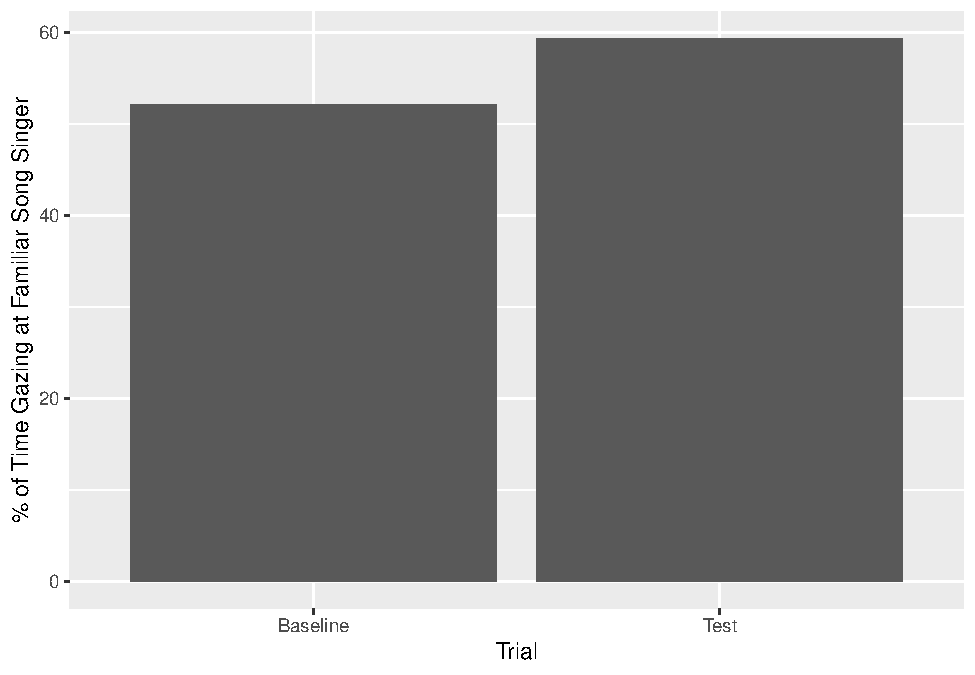
\includegraphics{APAReport_files/figure-latex/unnamed-chunk-5-1.pdf}

\hypertarget{discussion}{%
\section{Discussion}\label{discussion}}

The results showed that infants spent more time selectively paying attention to a novel person that sang a song that was familiar to the infant (as their parents had sang the same song) compared to chance, and compared to the amount of time the infant spent gazing at the same person before they sang the familiar song. These results suggest that song melodies may provide socially-relevant information to infants, specifically regarding whether a novel individual belongs to the same social environment as the infant.

\hypertarget{power-analysis}{%
\section{Power Analysis}\label{power-analysis}}

\begin{verbatim}
## Warning: package 'pwr' was built under R version 4.0.3
\end{verbatim}

\begin{verbatim}
## 
##      Paired t test power calculation 
## 
##               n = 32
##               d = 1
##       sig.level = 0.05
##           power = 0.9997799
##     alternative = two.sided
## 
## NOTE: n is number of *pairs*
\end{verbatim}

\begin{verbatim}
## 
##      Paired t test power calculation 
## 
##               n = 32
##               d = 0.43
##       sig.level = 0.05
##           power = 0.6541847
##     alternative = two.sided
## 
## NOTE: n is number of *pairs*
\end{verbatim}

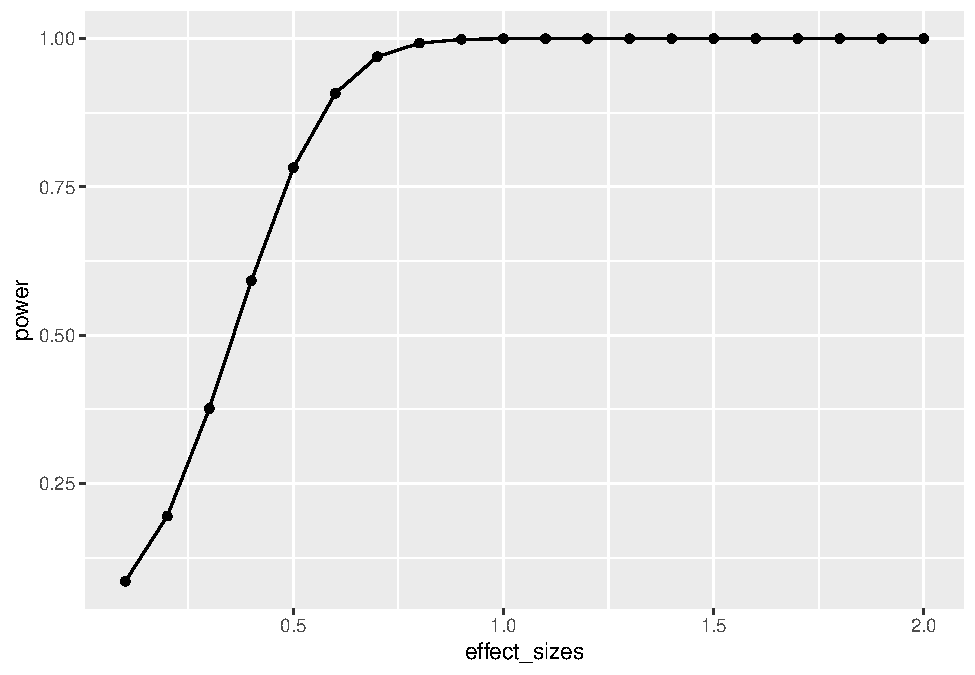
\includegraphics{APAReport_files/figure-latex/unnamed-chunk-6-1.pdf} 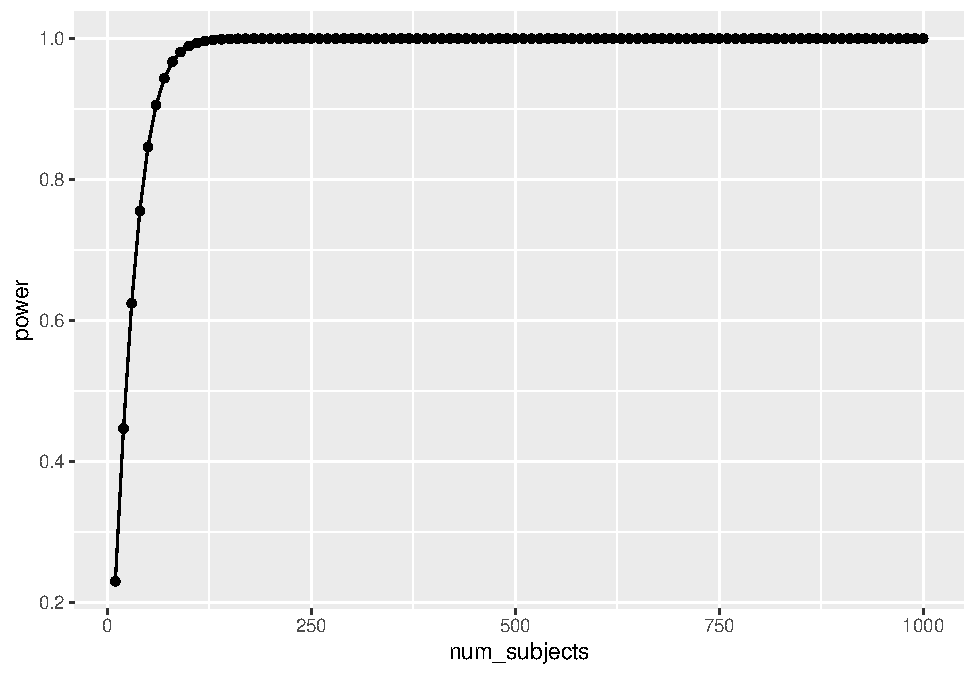
\includegraphics{APAReport_files/figure-latex/unnamed-chunk-6-2.pdf}

\begin{verbatim}
## 
##      Paired t test power calculation 
## 
##               n = 50
##               d = 0.43
##       sig.level = 0.05
##           power = 0.8462539
##     alternative = two.sided
## 
## NOTE: n is number of *pairs*
\end{verbatim}

I conducted a power analysis for the analysis comparing the proportion of time infants spent looking at the singer of the familiar song at the test trial (after she had sung the song), to the proportion of time the infants spent looking at the singer of the familiar song at the baseline trial (before she sung the song). Therefore, the power analysis conducted is for a paired-sample t-test. The assumptions were a sample size of 32 subjects (which was the sample size in the experiment), an effect size (Cohen's d) of 1, and a significance level set at .05. The calculation yielded a power of 0.9997799, which is essentially a power of 1. The authors had reported in their paper that they conducted a power analysis prior to conducting their experiment which yielded the target sample size of 32 participants in order to ensure adequate power to detect an effect. The authors cited another experiment with a similar design that tested the effects of language instead of music (Kinzler et al., 2007), and indicated that in this experiment, Kinzler and colleagues obtained an effect size of d=.54, and a sample of n=32 had .84 power to detect this effect. In the current experiment, Mehr and colleagues detected an effect size of d=.43. As this is a smaller effect size than that reported by Kinzler, Dupoux, and Spelke (2007), we would expect lower power to detect this effect, for the same sample size; indeed, when the power analysis is conducted with the parameters of a sample size of 32 subjects and an effect size of .43, the power is .654. This can also be seen in the power curve. As the effect size is lower than what was expected based on similar prior studies, the design may benefit from an increased sample size in order to increase the power to detect an effect size of this magnitude. As the authors were comfortable with a power of .84 for their experiment, in order to ensure this level of power for their obtained effect size of .43 (for example, if they were to replicate the experiment), based on a graph of power as an effect of sample size as well as a new power calculation, I would recommend a sample size of approximately 50 participants for future experiments that may try to replicate these results.

\newpage

\hypertarget{references}{%
\section{References}\label{references}}

\begingroup
\setlength{\parindent}{-0.5in}
\setlength{\leftskip}{0.5in}

\hypertarget{refs}{}
\leavevmode\hypertarget{ref-kinzler_native_2007}{}%
Kinzler, K. D., Dupoux, E., \& Spelke, E. S. (2007). The native language of social cognition. \emph{Proceedings of the National Academy of Sciences}, \emph{104}(30), 12577--12580. \url{https://doi.org/10.1073/pnas.0705345104}

\leavevmode\hypertarget{ref-mehr_for_2016}{}%
Mehr, S. A., Song, L. A., \& Spelke, E. S. (2016). For 5-Month-Old Infants, Melodies Are Social. \emph{Psychological Science}, \emph{27}(4), 486--501. \url{https://doi.org/10.1177/0956797615626691}

\endgroup


\end{document}
